\section{One big experiment}\label{sec:1}
Let $P = \num{10000}$ and $X = 1$. Since only one experiment is done,
\cref{eq:pi_final} cannot be used to calculate the uncertainty. Because of that
the uncertainty is defined as
\begin{equation}
	\Delta \pi_x = \sqrt{\text{Var}(4[X^2 + Y^2 \leq 1])}
    \label{eq:uncertainty_for_one_x}
\end{equation}
with $\text{Var}(X)$ being the variance of the random variable $X$.
Letting the experiment run results in a value of
\begin{equation}
	\pi_x = \num{3.1 \pm 1.7},
\end{equation}
which is considering the uncertainty of approximately \per{53} close to the real value.\par
%
When doing just one experiment, the distribution of the generated points is 
of interest. For this the histogram of the radii $R = \sqrt{X^2 + Y^2}$
and the squared radii are plotted in \cref{fig:radii_hist,fig:radii_squared_hist}.
For the radii we can see a linear rising distribution with a maximum at $r=1$, after which 
the distribution drops. 
The linear rise is explainable with the following argumentation:\\
The points generated inside the square are distributed uniformly, but since 
the circumference of a circle is proportional to the radius, the point density $n(r)$
also has to be $n(r)  \sim  r$. The drop after $r = 1$ occurs because 
a circle with radius $1$ is the biggest that fits inside a $2\times 2$ 
square, so there will be fewer points that can be generated with that radius and thus 
the distribution for $r > 1$ can be written as $n(r) \sim r(1-f(r))$ where 
the function $f(r)$. 
Let us think about a circle with a radius bigger than 1 and concentrate on 
and eighth of the circle. This is shown in \cref{fig:circle_square}. 
The part of the circle between the marked 0 and $\phi_\text{max}$
are outside the square. The value for $\phi$ in terms of the radius $r$ and the coordinate 
$x$ is 
\[
    \phi(r, x) = \arctan\qty(\frac{\sqrt{r^2 - x^2}}{x}).
\]
We see that $\phi(r, r) = 0$ and $\phi_\text{max} = \phi(r, 1) = \arctan\qty(\sqrt{r^2 - 1})$
for a square with a width of $2$. 
Since we have 8 such parts outside the square, the normalized distribution can be 
written as 
\[
    n(r) = \frac \pi 2 r (1 - f(r))
\]
with 
\[
    f(r) = \begin{cases}
        0 & r \leq 1 \\
        \frac 4\pi \arctan(\sqrt{r^2 - 1}) & 1 < r \leq \sqrt{2} \\ 
        1 & r > \sqrt 2
    \end{cases}
\]
because $n(r)$ has to be zero for $r > \sqrt 2$. 
In \cref{fig:radii_hist} the generated with the expected distribution are shown. 
Clearly they look very similar to each other.\par
%
\begin{figure}[h]
    \centering
    \importtikz{0.5\linewidth}{tikz/circle.tikz}
    \caption{A circle that is partly inside and partly outside a square.}
    \label{fig:circle_square}
\end{figure}
%
The $R^2$ distribution can be calculated from the $R$ distribution. For two random variables $X, Y$ and 
a function $V: X \rightarrow Y$ and given distribution $n(x)$, the distribution of 
$Y$ can be calculated with the dirac delta $\delta(x)$ by 
\[
    p(y) = \int_X dx\, n(x) \delta(y - V(x)).
\] 
For the variable $\rho = r^2$ we get 
\begin{align*}
    p(\rho) &= \frac \pi 2 \int_0^{\infty} dr\, r(1-f(r)) \delta(r^2 - \rho) \\
    &= \frac \pi 4 - 
    \begin{cases}
        0 & \rho \leq 1 \\
        \arctan(\sqrt{\rho - 1}) & 1 < \rho \leq 2 \\
        \frac{\pi}{4} & \rho > 2
    \end{cases}
\end{align*}
In \cref{fig:radii_squared_hist} it is shown that the data satisfies the expectation.\par 
The distribution of the indicator variable $\iv{X^2 + Y^2 \leq 1}$ is shown in \cref{fig:indicator}.
%
\begin{figure}[h]
    \centering
    \begin{subfigure}{.45\linewidth}
        \centering
        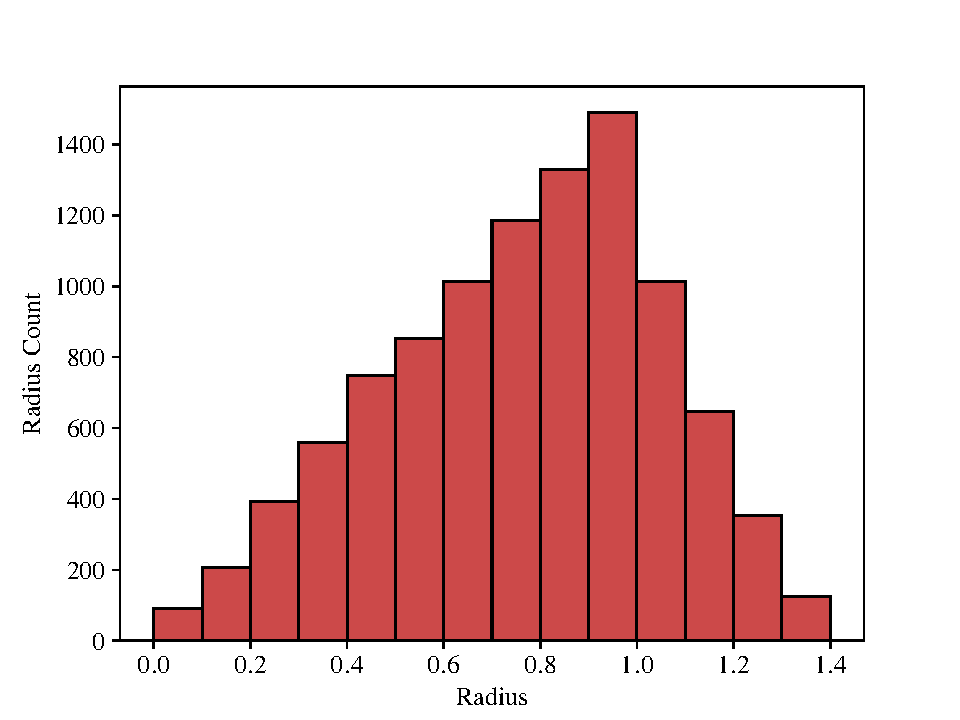
\includegraphics[width=\linewidth]{figs/ex1.1_radii_hist.pdf}
        \caption{Radii of generated points.}
        \label{fig:radii_hist}
    \end{subfigure}
    \hfill
    \begin{subfigure}{.45\linewidth}
        \centering
        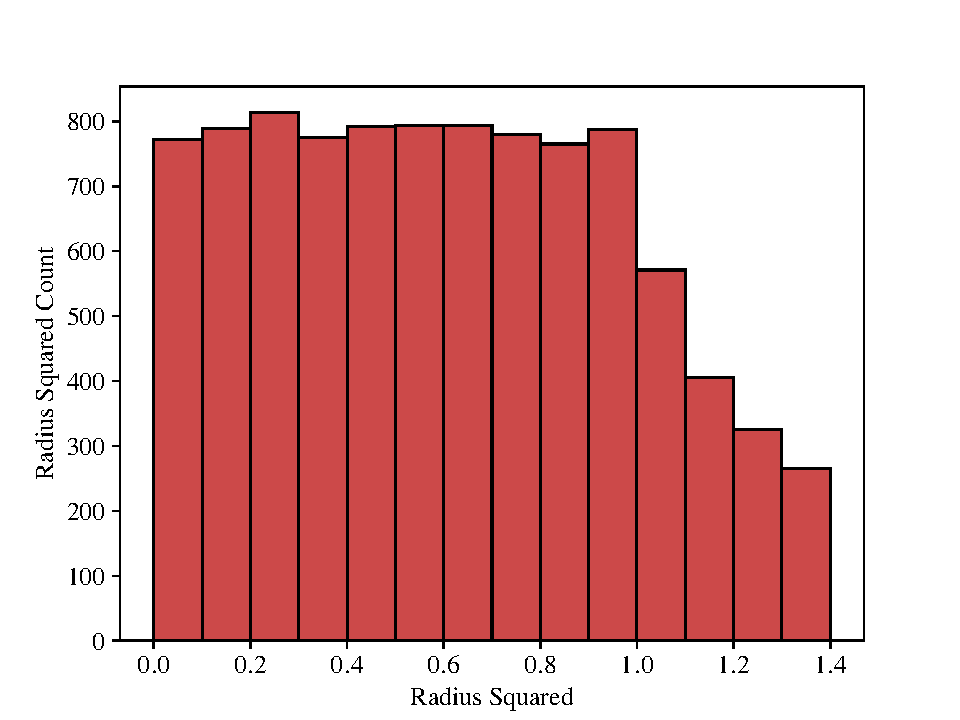
\includegraphics[width=\linewidth]{figs/ex1.1_radii_squared_hist.pdf}
        \caption{Squared radii of generated points.}
        \label{fig:radii_squared_hist}
    \end{subfigure}
    \caption{Normalized histograms of generated data with $P=\num{10000}$ 
    and $X = 1$ compared to expected distributions.}

\end{figure}
%
\begin{figure}[htbp]
    \centering
    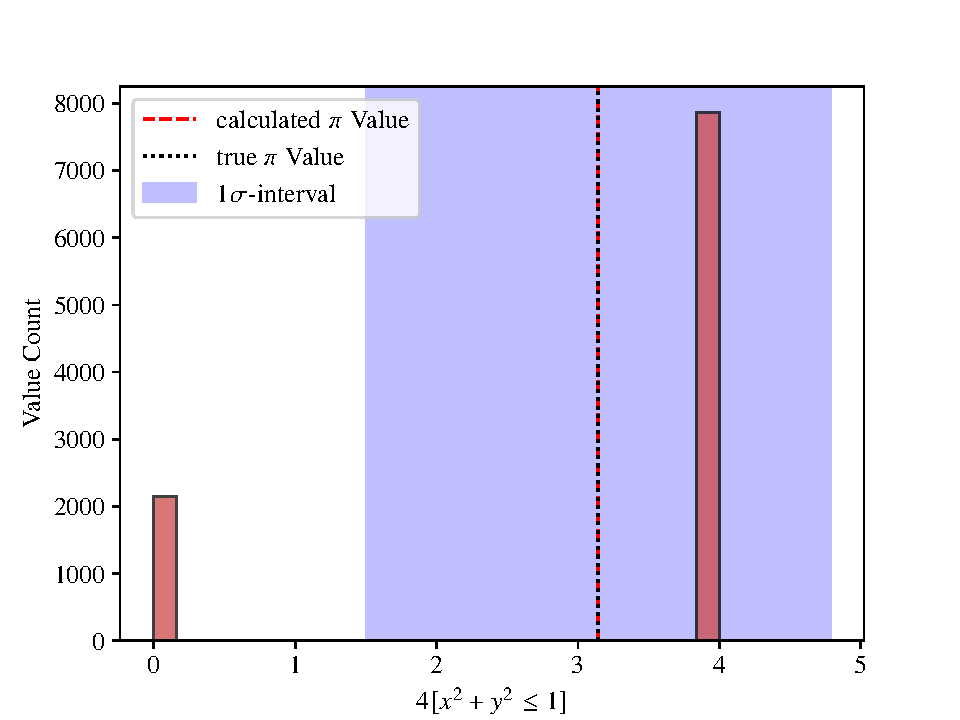
\includegraphics[width=.6\linewidth]{figs/ex1.1_indicator_hist.pdf}
    \caption{Histogram of the indicator variable $[X^2 + Y^2 \leq 1]$ for an experiment 
        with $P = \num{10000}$.}
    \label{fig:indicator}
\end{figure}